\documentclass[../thesis.tex]{subfiles}

\begin{document}

\chapter{Decision Support Tool for Multi-Hospital Planning of Frail and Elderly Resource Capacities}\label{chp:tool}

\section{Introduction}
This chapter will provide a tutorial guide on how to use the two tools discussed within Chapters \ref{chp:Experimental Analysis} and \ref{chp:Linking}. These tools are adaptable so can be applied to other health boards and scenarios or other patient groupings. Section \ref{sec:excelimp} will discuss the Microsoft Excel OpenSolver Tool which is specific to ABUHB. This model and approach can be replicated and applied to any other health board. Section \ref{sec:pythonimpl} discusses the Python PuLP implementation of the model, which can be generalised to any health board situation.


\section{Excel Implementation}\label{sec:excelimp}
Microsoft Excel is a widely used tool for data analysis and management, and OpenSolver is a powerful optimisation engine that can be used to solve complex problems within Excel. In this guide, we will provide step by step instructions on how to run the OpenSolver model, from setting up your data and formulating your problem to running the optimisation and analysing the results.

The OpenSolver model without the ABUHB data has been provided on GitHub \cite{Williams2023} to allow users to enter their own data and hospital specialties. Each type of parameter has its own individual sheet and is clearly named to ensure the planners can easily access data. Due to the limitations of the software, all decision variables in the optimisation model must be on the same sheet. For visualisation purposes, the decision variables are automatically transferred into the model sheets after the experiment has run.

\subsection*{Data}
Figure \ref{fig:exdata} displays the data which is used by the model. This is stored within the `Data' tab and allows users to enter and change the parameters to suit their model. The user is required to enter the hospital and specialty into which a patient is admitted. The `Short LOS' determines the number of nights spent in hospital, whilst the `LOS\_hours' determines the continuous time spent in hospital. Additionally, the date column can be added if the user wishes to split their model by year, season, month or days of the week. Finally, there is the NHS Patient Identifier which is unique to the patient.

\begin{figure}[h!]
    \centering
    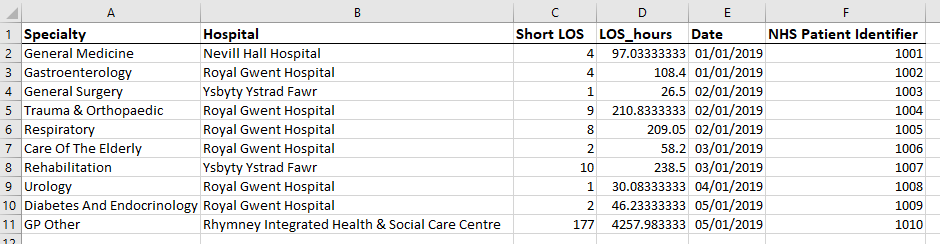
\includegraphics[width=\textwidth]{Chapters/Chapter7/Figures/Data.png}
    \caption{The data requirements for the Excel OpenSolver plugin where the user is required to enter, as a minimum, the `Specialty', `Hospital' and either `Short LOS' or `LOS\_hours' for each patient.}
    \label{fig:exdata}
\end{figure}


\subsection*{Demand}
The demand for each specialty is automatically generated from the data inputted by the user and is stored in the `Demands' tab within the Excel spreadsheet. The average demand is calculated by determining if a specialty and hospital combination is present, and if so, calculating the total. Similarly, if patients do fall within these combinations then the average LOS, using `LOS\_hours', is calculated for each specialty and hospital. These values are then multiplied together and subsequently divided by 24, as the LOS is given in hours, and then by the total number of days in the data, to give a daily demand. This means if a user wants to determine a monthly demand, the `Number of Days in Data' can be changed to the number of months within the data. This is then stored as a table shown in Figure \ref{fig:exdemand}.
\begin{figure}[h!]
    \centering
    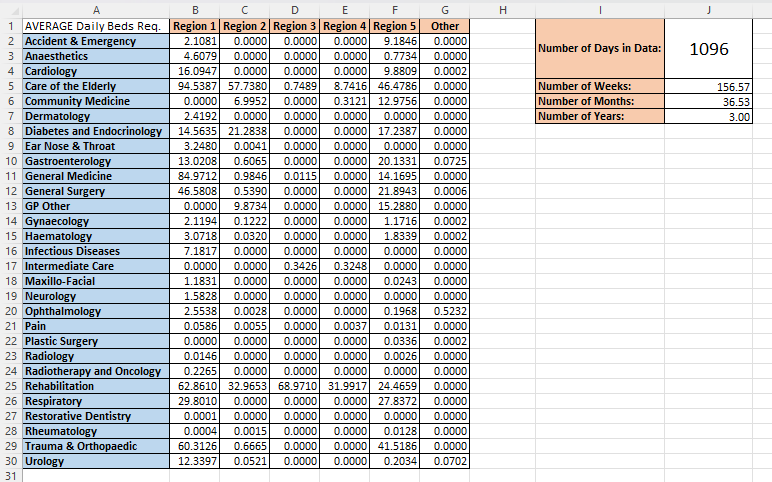
\includegraphics[width=\textwidth]{Chapters/Chapter7/Figures/Demands.png}
    \caption{The average daily bed demand matrix automatically generated by Excel, segmented by region and specialty. The user is required to enter the number of days within the data.}
    \label{fig:exdemand}
\end{figure}

\subsection*{Possible Hospital Locations}
The tab entitled `Hospital-Specialty' contains data regarding whether a hospital is able to open a specialty. In order to restrict the number of beds that can be deployed in a hospital's location, the total bed capacity for the 1$^{st}$ and 2$^{nd}$ stages of the model can be seen within Figure \ref{fig:exlocations}. As some hospitals may not be able to open full capacity to one specialty, due to resource or space limitations, the user is able to reduce these values whilst still being able to open up to the full capacity across other specialties. If a value of zero is present, this means the hospital is unable to open that specialty.
\begin{figure}[h!]
    \centering
    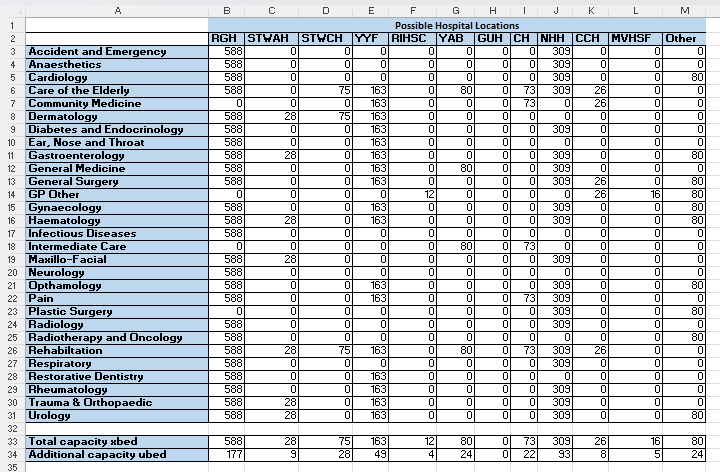
\includegraphics[width=\textwidth]{Chapters/Chapter7/Figures/Hospital-Spec.png}
    \caption{The maximum number of beds that can be deployed to each hospital location for each specialty. Additionally, the user is required to enter the total capacity for the hospitals in the first and second stages.}
    \label{fig:exlocations}
\end{figure}

\subsection*{Hospital Costs}
Within the `Hospital Costs' tab in the spreadsheet, the user is able to enter the average daily cost for each specialty. Similar to demands, if the user wants to work in a different time frame; monthly, seasonally, or yearly, the cost figures can also be adjusted. Figure \ref{fig:excostings} displays the 1$^{st}$ stage hospital costs, with an identical matrix grid being found below in the spreadsheet for the 2$^{nd}$ stage costs. 
\begin{figure}[h!]
    \centering
    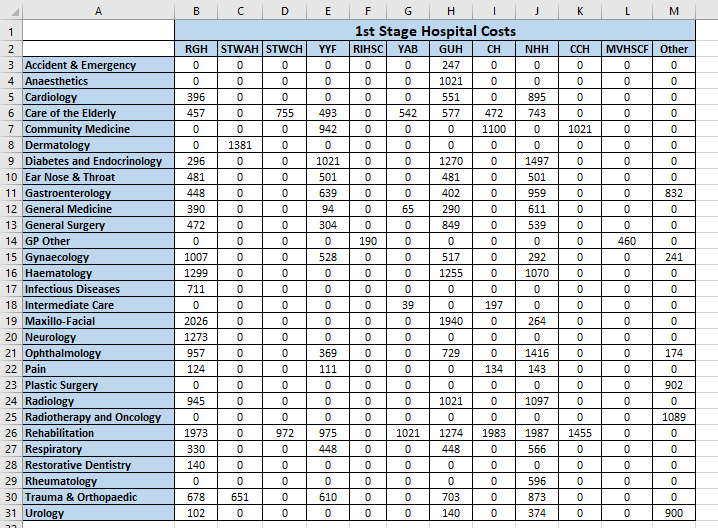
\includegraphics{Chapters/Chapter7/Figures/Costings.png}
    \caption{The user is required to enter the first stage cost for each hospital and specialty combination.}
    \label{fig:excostings}
\end{figure}

\subsection*{Staffing}
The `Staffing' tab in the Excel worksheet contains all the necessary information for the staffing requirement. Firstly, the staff to patient ratio can be altered depending on the band level and the specialty (Figure \ref{fig:exstaff}). The hourly and daily cost per member of staff can also be changed. This flexibility allows pay rises to be included and flexibility in costings across other countries. Similarly, the cost of NHS bank and agency staff was also included. Finally, the maximum number of staff that can be deployed both in the first and second stages is detailed. 

One limitation of the Excel model is higher levels of staff cannot perform the role of the lower band staff members. This is due to the non-linearity of the constraint which the COIN-OR CBC (Linear solver) cannot handle.

\begin{figure}[h!]
    \centering
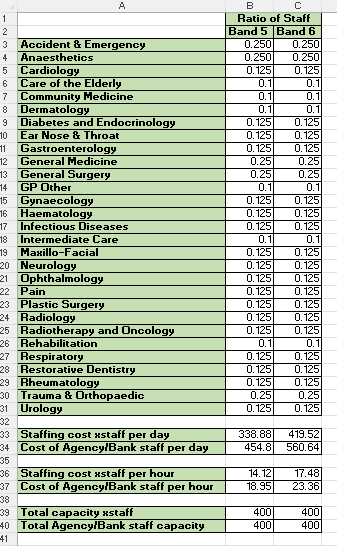
\includegraphics{Chapters/Chapter7/Figures/exStaff.png}
    \caption{The user is required to enter the ratio of nursing band staff to each specialty. Additionally, the user is required to enter the cost per hour of the first and second stage nurses staff, and the total capacity.}
    \label{fig:exstaff}
\end{figure}

\subsection{Deterministic Model}
The deterministic model is stored within the `Deterministic' tab, where the optimisation model can be run and the results analysed. With the OpenSolver add-in installed, the model can be easily accessed through the Data ribbon and then selecting the Model on the OpenSolver toolbar. This brings up Figure \ref{fig:exdmos}, which depicts the objective function cell, the type of problem (maximisation or minimisation), the decision variables, the model's constraints and the type of solver engine. Using the options button; the maximum solution time, branch and bound tolerance and the maximum number of iterations can also be changed. To solve the model, the `Solve' button can be selected on the OpenSolver toolbar.

\begin{figure}[h!]
    \centering
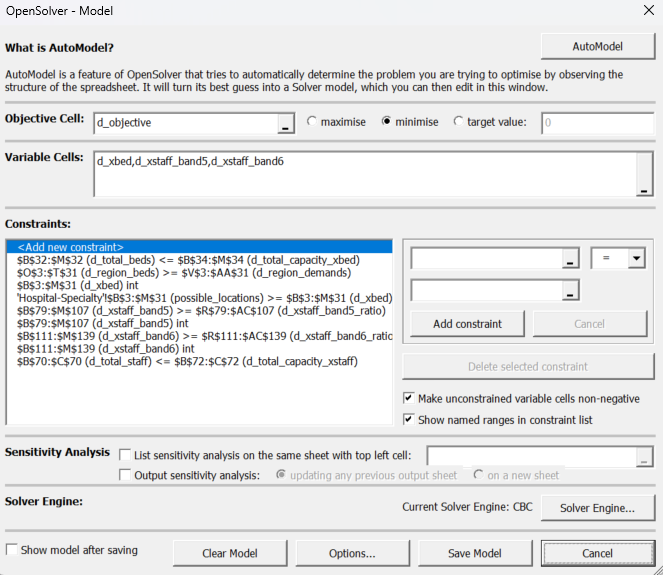
\includegraphics[width=\textwidth]{Chapters/Chapter7/Figures/DeterministicOS.png}
    \caption{The OpenSolver objective cell, decision variable cells and constraints for the deterministic implementation. The `Current Solver Engine' can be changed to Gurobi if a license is available.}
    \label{fig:exdmos}
\end{figure}
Once executed, the total cost of the model is shown within the sheet, along with the total number of beds and staff to be deployed (Figure \ref{fig:exdm1a}). The model shows where each of these beds should be deployed across the specialties and hospitals, and the overall number of beds within each hospital. Similarly, the number of staff deployed for each band can be visualised within the same worksheet, as shown in Figure \ref{fig:exdm2a}.

\begin{landscape}
\begin{figure}[h!]
    \centering
    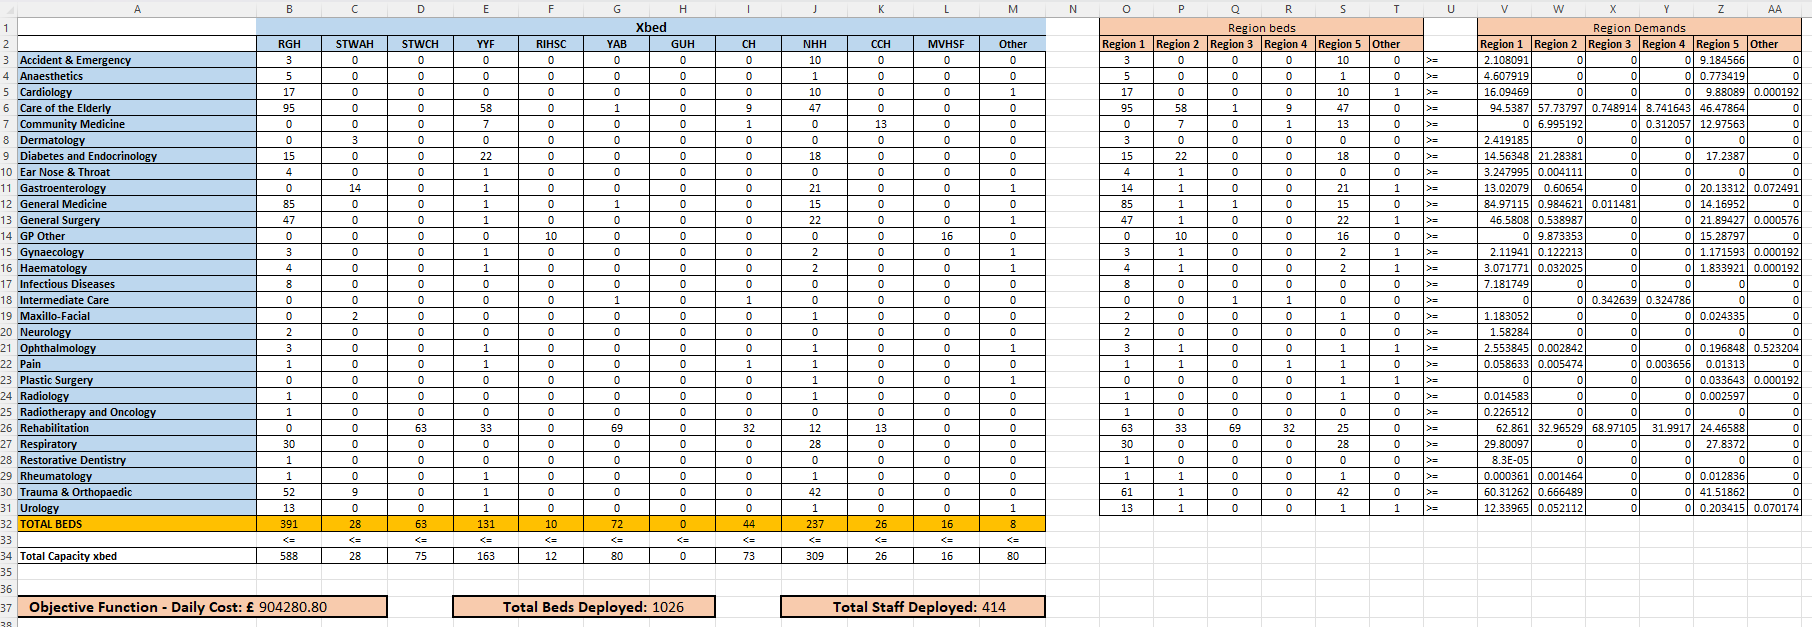
\includegraphics[scale=0.7]{Chapters/Chapter7/Figures/Deterministic1.png}
    \caption{The output from the deterministic model once solved, displaying the number of beds to deploy to each hospital and specialty. The total daily cost, beds and staff are also summarised. }
    \label{fig:exdm1a}
\end{figure}
\end{landscape}
\begin{figure}[h!]
    \centering
    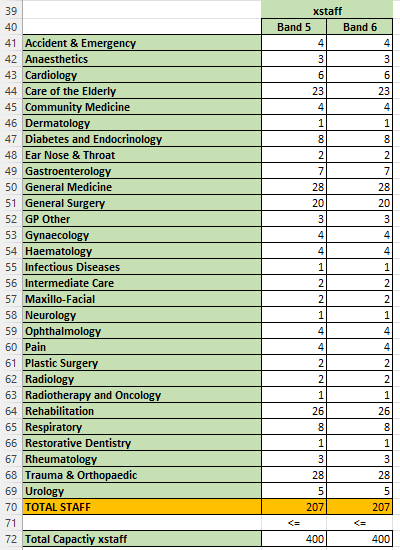
\includegraphics[scale=0.8]{Chapters/Chapter7/Figures/deterministic2.png}
    \caption{The staffing output from the deterministic model once solved, displaying the number of nursing staff to deploy to each specialty and of which band level.}
    \label{fig:exdm2a}
\end{figure}

\subsection{Two-Stage Stochastic Model}
The two-stage stochastic model is stored within the `Stochastic' tab. Due to the large number of decision variables within the stochastic model (6,960 variables), the model is stored within `SVariables' and the results are automatically transferred into the `Stochastic' tab.

In addition to the deterministic model parameters, the scenarios and probabilities for each scenario are required. The Excel tool can use up to four scenarios by changing the values as demonstrated in Figure \ref{fig:exscen}.
\begin{figure}[h!]
    \centering
    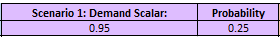
\includegraphics{Chapters/Chapter7/Figures/scenarios.png}
    \caption{The scenario selector for the two-stage stochastic implementation. Users are prompted to input the demand scalar and the corresponding probability of occurrence.}
    \label{fig:exscen}
\end{figure}

Similar to the deterministic model, the stochastic model's constraints can be seen within the `Data' ribbon and selecting the `Model' option. Figure \ref{fig:exdm2} shows the objective function cell, as well as the decision variable locations. The stochastic model contains 31 constraints, as well as the option to make unconstrained variable cells non-negative. Once again, the COIN-OR CBC linear solver or the Gurobi can be used.

\begin{figure}[h!]
    \centering
    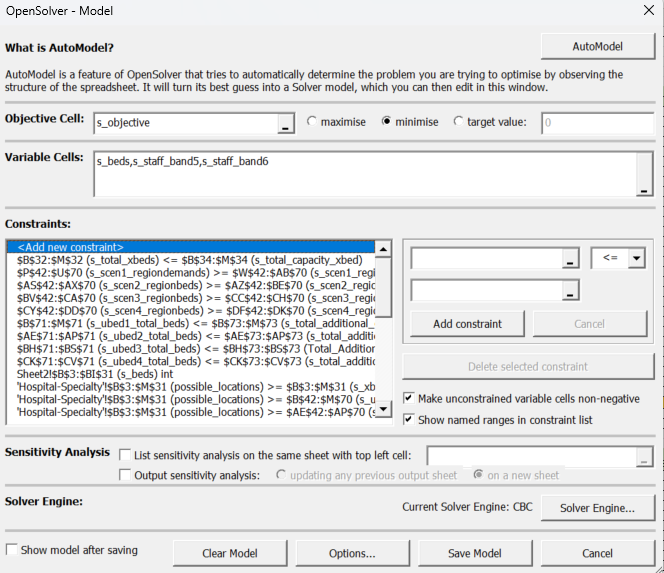
\includegraphics[width=\textwidth]{Chapters/Chapter7/Figures/Stochastic2.png}
    \caption{The OpenSolver objective cell, decision variables and constraints for the two-stage stochastic implementation. The `Current Solver Engine' can be changed to Gurobi if a license is available.}
    \label{fig:exdm2}
\end{figure}
Once the model has run, the output produced is similar to the one shown in Figure \ref{fig:exdm1}. The model determines how many beds and staff to deploy in the first and second stages to ensure the minimum demand is met. A summary is provided within rows 37 and 38 on the worksheet, but the full breakdown of the results can be seen within the remainder of the worksheet.

\begin{figure}[h!]
    \centering
    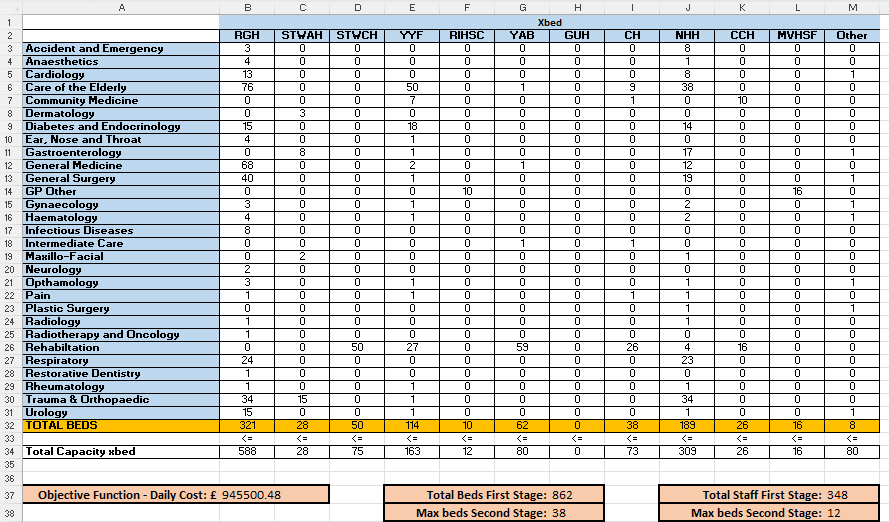
\includegraphics[width=\textwidth]{Chapters/Chapter7/Figures/Stochastic1.png}
    \caption{The output from the two-stage stochastic model once solved, displayed the number of beds to deploy to each hospital and specialty. The total daily cost, first and second stage beds and nursing staff are also summarised.}
    \label{fig:exdm1}
\end{figure}


\subsection{Test A}
Test A is stored in the `TestA' tab, where the optimisation model can be run and the results analysed. Similar to the stochastic model, due to the large number of decision variables within the optimisation model, the model is stored within `OVariables' and the results are automatically transferred into the `TestA' tab.

For Test A, the first stage of the model is required to be fixed to the results of the deterministic model. The Excel spreadsheet has been setup in a way that requires no additional user input is required for this Test. This is achieved by linking the cells together, i.e., \texttt{=Deterministic!B3}, which would copy the first hospital and specialty into the first stage of the model.

Similar to the previous two models, the constraints can be seen within the `Data' ribbon and selecting the `Model' option. Figure \ref{fig:testA} displays the output of the model, showing a summary of the daily costing figures as well as the numbers of beds and staff deployed in the first and second stages.

\begin{figure}[h!]
    \centering
    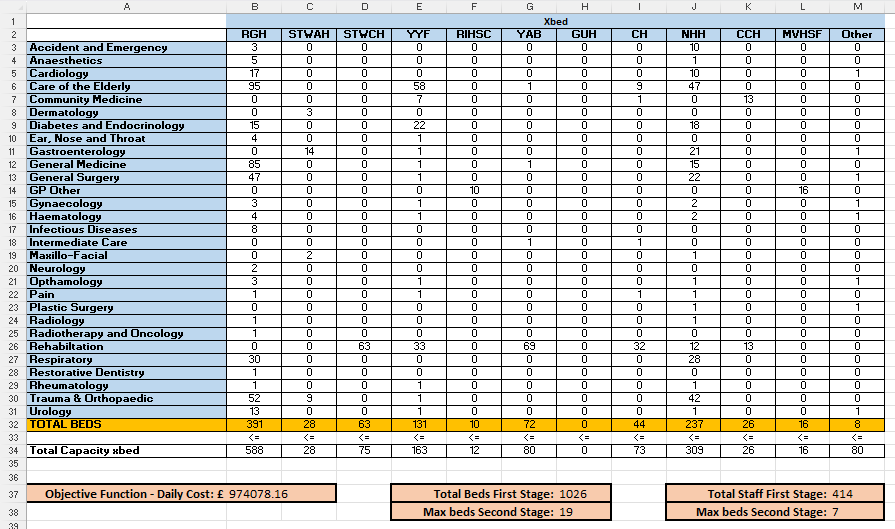
\includegraphics[width=\textwidth]{Chapters/Chapter7/Figures/TestA.png}
    \caption{The output from Test A model implementation once solved, displayed the number of beds to deploy to each hospital and specialty. The total daily cost, first and second stage beds and nursing staff are also summarised.}
    \label{fig:testA}
\end{figure}

\subsection{Test B}
Test B is stored in the `TestB' tab of the workbook, and its purpose is to determine if the correct first stage variables have been chosen. 

This test requires the zero or lowest value stage variables of the deterministic model to be set to zero or the lower bound. As some specialties cannot open within certain hospitals of ABUHB, this means there will always be zero variables, and therefore the model is setup in a way to determine if zero beds are deployed in the deterministic model, then it will return zero. Otherwise, it will return the maximum number of beds that can be opened within the hospital.
An example of how this is generated is as follows: \texttt{IF(Deterministic!B3=0, 0, `Hospital-Specialty'!B3)}, where cell \textttt{B3} is the first hospital/specialty combination. The formula checks the `Deterministic' tab to determine whether or not the B3 cell is 0, if so, then a zero is placed into the cell. If not, the value from the corresponding cell in the `Hospital-Specialty' tab is taken.

If there was a scenario in which, all specialties in all hospitals had been opened, the user would have to manually enter the lower bound.

The results of the `IF statement' are then outputted into cells \texttt{AB3:AM31} (Figure \ref{fig:TestB}). As OpenSolver works with the linear programming add-in, the `IF statement' causes this to become non-linear. To overcome this, the user is required to copy and paste cells \texttt{AB3:AM31} into \texttt{O3:Z31} ensuring only the values and not the formulae are copied over.

Figure \ref{fig:testbconstraint} illustrates the additional constraint necessary for the model to run successfully. To access this constraint, along with the other constraints, the user can select the `Data' ribbon and the `Model' option. The output from the model, showing the objective function and bed and staff totals can be seen in Figure \ref{fig:testBfin}.

\begin{figure}[h!]
    \centering

\includegraphics{Chapters/Chapter7/Figures/TestBconstraint.png}
    \caption{The additional constraint required for Test B, where the zero variables within the deterministic model are set as the lower bound for the first stage within Test B.}
    \label{fig:testbconstraint}
\end{figure}

\begin{landscape}
\begin{figure}
    \centering
    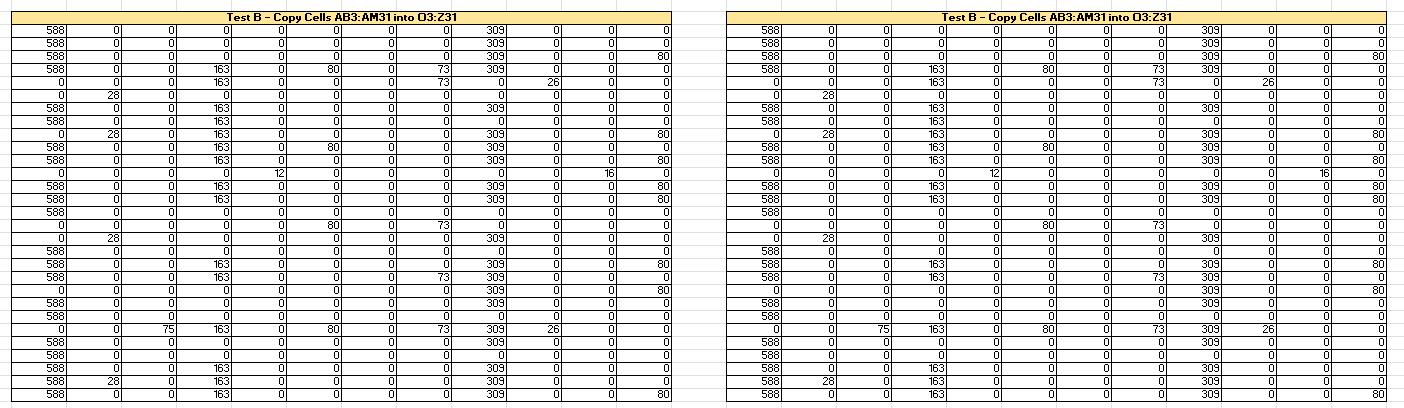
\includegraphics[scale=0.65]{Chapters/Chapter7/Figures/TestB.png}
    \caption{For Test B, an `if statement' is required to be used to determine the zero bound of the decision variables from the Deterministic output. As OpenSolver is a linear programming solver, the user is required to copy and paste the values only from cells \texttt{AB3:AM31} to \texttt{O3:Z31}.}
    \label{fig:TestB}
\end{figure}
\end{landscape}

\begin{figure}[h!]
    \centering
    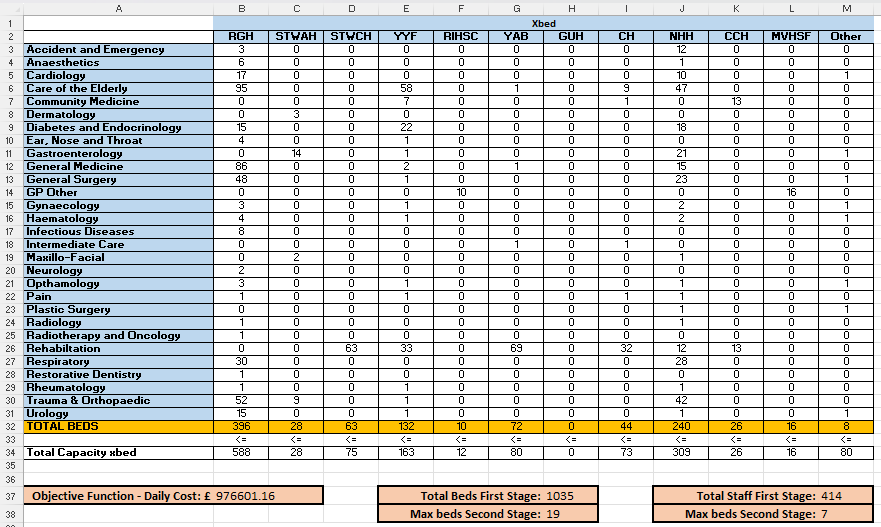
\includegraphics[width=\textwidth]{Chapters/Chapter7/Figures/TestBfin.png}
    \caption{The output from Test B model implementation once solved, displayed the number of beds to deploy to each hospital and specialty. The total daily cost, first and second stage beds and nursing staff are also summarised.}
    \label{fig:testBfin}
\end{figure}



\subsection{Test C}
Test C is stored in the `TestC' tab of the workbook and its purpose is to determine the upgradeability of the model. Similar to Test A, the Excel spreadsheet has been set up in a way that requires no additional user input. An example of how this is achieved is as follows: \texttt{=Deterministic!B3} which will copy the first hospital and specialty. 

This results in the following matrix to be inputted into cells \texttt{O3:Z31}, as shown in Figure \ref{fig:TestC}.

\begin{figure}
    \centering
    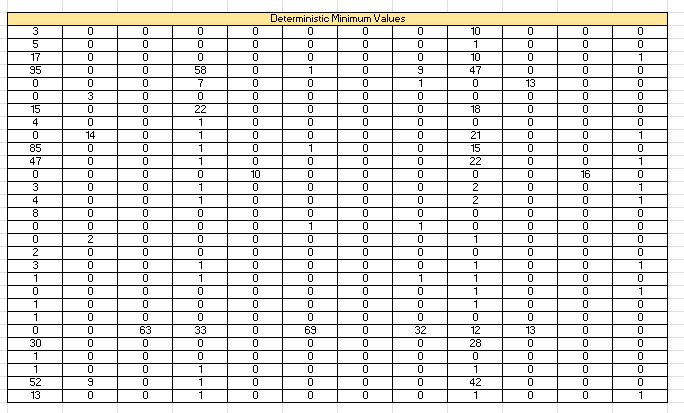
\includegraphics[width=\textwidth]{Chapters/Chapter7/Figures/TestC.png}
    \caption{The minimum values which are required to be met within the first stage of Test C. This will determine the upgradeability of the model.}
    \label{fig:TestC}
\end{figure}

Therefore an additional constraint to the original two-stage stochastic model is added into the constraint list to ensure the first stage variables meet the minimum deterministic values. The constraint is shown in Figure \ref{fig:testCcon}.

\begin{figure}
    \centering
    
\includegraphics{Chapters/Chapter7/Figures/TestCcon.png}
    \caption{The additional constraint required for Test C, where the deterministic values are the minimum bound for the first stage of Test C.}
    \label{fig:testCcon}
\end{figure}

The remainder of the model remains the same as the two-stage stochastic deployment and the output of the results can be seen as exampled in Figure \ref{fig:testcfin}.

\begin{figure}
    \centering
    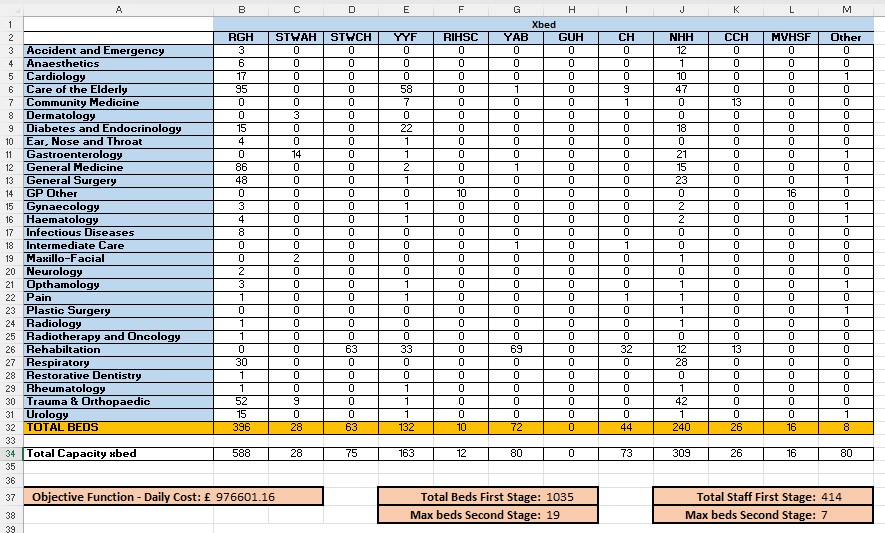
\includegraphics[width=\textwidth]{Chapters/Chapter7/Figures/TestCfin.png}
    \caption{The output from the deterministic model once solved, displaying the number of beds to deploy to each hospital and specialty. The total daily cost, beds and staff are also summarised. }
    \label{fig:testcfin}
\end{figure}

\newpage
\section{Python Implementation}\label{sec:pythonimpl}
Python is a high-level programming language that can be used for a wide range of applications such as web development, data analysis, scientific computing, artificial intelligence, and automation. In this guide, a step by step tutorial is provided and the input requirements of the user will be discussed. 

The deterministic and two-stage stochastic optimisation models have been provided on GitHub \cite{Williams2023} to enable users to apply this to their own scenario. The model requires users to install the PuLP package \cite{Mitchell2019}, and these models were developed using PuLP version 2.3. Python contains a library named `itertools', which is also required. If the user has a Gurobi license, then this also requires importing into Python. For the models to run, these two libraries are required to be imported, as follows:

\begin{lstlisting}[language = python]
import pulp
import itertools
import gurobipy
\end{lstlisting}

\subsection{Deterministic Model}
The Python models use functions to pass data through and stores variables until later required. The first function initialises the problem and sets the decision variables. The `pulp.LpProblem' class creates a new linear programming problem with the name used within the output .lp file and the sense of the objective, whether this be a minimisation or maximisation. The `Lp.Variable' term creates the decision variables and stores them within a dictionary. The lower bound of the variables is set to zero to ensure there are no non-negative constraints, and the values are set to integer. In this case, the `xbed' variable is a two variable dictionary and the `xstaff' is a three variable dictionary.

\begin{lstlisting}[language = python]
def initialise_deterministic_minimisation_problem(
    specialties, hospitals, bands
):
    """
    Initialise the mininmisation problem. 
    Set decision variables for the models.
    """
    sh = [(s,h) for s in specialties for h in hospitals]
    shb = [(s,h,b) for s in specialties for h in hospitals for b in bands]

    prob = pulp.LpProblem("Deterministic", pulp.LpMinimize)
    
    xbed = pulp.LpVariable.dicts(
        "Xbed", (specialties, hospitals), lowBound=0, cat='Integer'
    )
    xstaff = pulp.LpVariable.dicts(
        "Xstaff", (specialties, hospitals, bands), lowBound=0,cat='Integer'
    )
    return prob, sh, shb, xbed, xstaff
\end{lstlisting}
Once the model is initialised, the deterministic constraints as listed in Section \ref{sec:deterministicmodel}, can be inputted into the model. The deterministic model in total contains 10 constraints. PuLP uses the assignment operator `+=', to store the results of an expression to the `prob' term. The class `lp.Sum' is used to sum the list of linear expressions. For loops are used to cycle through all the elements in the list. This can be seen as follows in the `add\_deterministic\_constraints' function:
\begin{lstlisting}[language = python]
def add_deterministic_constraints(xbed, xstaff, UBbed, UBstaff, D, K, R, sh, shb, prob):
    """
    Add the constraints that are required for the deterministic model
        
    - Constraints 1-6: Ensures demand is met across all specialties and all regions
    - Constraint 7: Ensures beds are only able to open in a ward if the facilities are able to be opened 
    - Constraint 8: Ensures staffing ratios are met
    - Constraint 9: Ensures beds deployed does not exceed maximum capacity of hospital
    - Constraint 10: Ensures staff deployed does not exceed maximum staffing resources
    """
    
    for s in specialties:
        prob += pulp.lpSum(xbed[s][h] for h in region1) >= pulp.lpSum(D[s][0]) #Constraint 1
        prob += pulp.lpSum(xbed[s][h] for h in region2) >= pulp.lpSum(D[s][1]) #Constraint 2
        prob += pulp.lpSum(xbed[s][h] for h in region3) >= pulp.lpSum(D[s][2]) #Constraint 3
        prob += pulp.lpSum(xbed[s][h] for h in region4) >= pulp.lpSum(D[s][3]) #Constraint 4
        prob += pulp.lpSum(xbed[s][h] for h in region5) >= pulp.lpSum(D[s][4]) #Constraint 5
        prob += pulp.lpSum(xbed[s][h] for h in region6) >= pulp.lpSum(D[s][5]) #Constraint 6
        
        for h in hospitals:
            prob += pulp.lpSum(xbed[s][h])<= pulp.lpSum(K[s][h]) # Constraint 7
                
            for b in bands:
                prob += pulp.lpSum(xstaff[s][h][b]) >= pulp.lpSum(R[s][b]*(xbed[s][h])) #Constraint 8
            
    for h in hospitals:
        prob += pulp.lpSum(xbed[s][h] for s in specialties) <= UBbed[h]  #Constraint 9
        
    for b in bands:
        prob += pulp.lpSum(xstaff[s][h][b] for (s,h) in sh) <= UBstaff[b] # #Constraint 10
        
    return prob
\end{lstlisting}

The final function solves the deterministic model by calling all the previous functions. This is where the objective function of the model is defined and has to satisfy the constraints, which are called from the previous function. The model is solved using the `prob.solve()' term, where the solver; COIN-OR CBC linear solver, is selected. The `maxSeconds' determines the maximum time for the solver in seconds, whilst the `fracgap' sets the tolerance for the solver to stop.

\begin{lstlisting}[language= python]
def solve_deterministic_minimisation_problem(
    specialties,
    bands,
    hospitals,
    regions,
    D,
    K,
    R,
    cbed,
    cstaff,
    UBbed,
    UBstaff,
):
   
    """
    Solves the deterministic problem, with the objective function being minimised.
    """
    prob, sh, shb, xbed, xstaff = initialise_deterministic_minimisation_problem(
        specialties=specialties, 
        hospitals=hospitals, 
        bands=bands
    )
    
    prob += (
        pulp.lpSum((xbed[s][h] * cbed[s][h]) for (s,h) in sh) +
        pulp.lpSum((xstaff[s][h][b]*cstaff[b]) for (s,h,b) in shb)
    )
    
    prob = add_deterministic_constraints(
        xbed=xbed, 
        xstaff=xstaff, 
        UBbed=UBbed, 
        UBstaff=UBstaff,
        D=D, 
        K=K,
        R=R,
        sh=sh,
        shb=shb,
        prob=prob,
    )
    # The user can select one of the two optimisers:
    # prob.solve(pulp.GUROBI())
    # prob.solve(pulp.PULP_CBC_CMD())
    return prob
  
\end{lstlisting}
The values for the parameters are then required to be entered by the user. The total number of specialties, bands and regions can be entered manually and using the itertools package, lists are created. For each region, the hospitals are inputted into each array. For example, if region one had the first three hospitals the line `region1 = [0,1,2]' would be displayed. All regions are then summed together to determine the total number of hospitals within the health board. A two-dimensional demand array, D, is required by the user. Each row represents a specialty and each column represents the region. Similarly, the K value depicting how many beds can be deployed within each specialty and each hospital can also be inputted. Again, each row represents a specialty, with the column representing the hospital. Next, the ratios of each band of staff to specialty is required. The row of the array is representing specialty and the columns represent each band of nurse. The variable `cbed' relates to the cost of a bed per specialty in each hospital. The structure of this is identical to the K array. The `cstaff' parameter is a one-dimensional matrix where each entry relates to the cost of each band of nurse. Similarly, the `UBstaff' parameter is the maximum number of nurses for each band that are able to be deployed. Finally, the `UBubed' is the maximum number of hospital beds that can be deployed and each entry represents each hospital. The user can select one of the two solvers, either the CBC\_CMD solver: \texttt{prob.solve(pulp.PULP\_CBC\_CMD())} or the Gurobi solver: \texttt{prob.solve(pulp.GUROBI())}.
   

\begin{lstlisting}[language= python]
    """
    These values can be altered to the specific requirements of the user
    """
    specialties = list(itertools.chain(range(0, ))) #Creates list of specialties
    bands = list(itertools.chain(range(0, ))) #Creates list of nursing bands
    regions = list(itertools.chain(range(0, ))) #Creates List of regions

    region1 = []
    region2 = []
    region3 = []
    region4 = []
    region5 = []
    region6 = []
    hospitals = region1 + region2 +region3 + region4 +region5 +region6
    D = [ 
    [],
    ]
    K = [
    [],
    ]
    R = [
    [],
    ] 
    cbed = [
    [],
    ]
    cstaff = []
    UBstaff = [
    [],
    ]
    UBbed =[
    [],
    ]
\end{lstlisting}

In order for the optimisation to be solved, the user entered parameters are required to be fed into the model. This is computed by the following code:
\begin{lstlisting}[language=python]
    """
    Feeds the parameters into the deterministic optimisation model
    """
    prob = solve_deterministic_minimisation_problem(
    specialties,
    bands,
    hospitals,
    regions,
    D,
    K,
    R,
    cbed,
    cstaff,
    UBbed,
    UBstaff,
)
\end{lstlisting}
In order to ensure the model has been solved, LpStatus, returns the status of the problem, either suggesting an optimal solution has been found or the model is infeasible. The total objective function can also be displayed using the `value' parameter. To display all non-zero decision variables, a `for' loop has been created which prints out the decision variable name along with the number of beds or staff to deploy.

\begin{lstlisting}[langauge=python]
    print("Solution Status = ", pulp.LpStatus[prob.status])
    print("Total price = ", pulp.value(prob.objective))  
    for v in prob.variables():
        if v.varValue >= 0:
            print(v.name, "=", v.varValue)
\end{lstlisting}

\subsection{Two-Stage Stochastic Model}\label{sec:pystochmod}
The two-stage stochastic model follows a similar structure to the deterministic model with similar functions used to develop the model. Within this section, the differences between the two models will be discussed. The first function is named the `initialise\_stochastic\_minimisation\_problem' where the first and second stage decision variables are set and the problem is initialised. The second stage variable `ubed' is a three variable dictionary which includes specialties, hospitals and bands. The `ustaff' decision variable is a four variable dictionary with parameters specialties, hospitals, bands and scenarios.
\begin{lstlisting}[language=python]
def initialise_stochastic_minimisation_problem(
    specialties, hospitals, bands, regions, scenarios
):
    """
    Initialise the minimisation problem.
    Set decision variables for the models.
    """
    sh = [(s,h) for s in specialties for h in hospitals]
    shb = [(s,h,b) for s in specialties for h in hospitals for b in bands]
    shk = [(s,h,k) for s in specialties for h in hospitals for k in scenarios]
    srhk = [(s,r,h,k) for s in specialties for r in regions for h in hospitals for k in scenarios]
    sbhk = [(s,b,h,k) for s in specialties for b in bands for h in hospitals for k in scenarios]
    
    prob = pulp.LpProblem("Stochastic", pulp.LpMinimize)
    
    xbed = pulp.LpVariable.dicts(
        "Xbed", (specialties,hospitals), lowBound=0, cat = 'Integer'
    )
    xstaff = pulp.LpVariable.dicts(
        "Xstaff", (specialties,hospitals,bands), lowBound=0,cat = 'Integer'
    )
    ubed = pulp.LpVariable.dicts(
        "Ubed",(specialties,hospitals,scenarios), lowBound=0, cat='Integer'
    )
    ustaff = pulp.LpVariable.dicts(
        "Ustaff",(specialties,hospitals,bands,scenarios), lowBound=0, cat='Integer'
    )
    return prob, sh, shb, shk, srhk, sbhk, xbed, xstaff, ubed, ustaff
\end{lstlisting}

The two-stage stochastic modelling constraints as generated in Section \ref{sec:stochasticmodel}, can be initialised into the model. The two-stage stochastic model has a total of 14 constraints, an additional four compared to the deterministic model. Constraint 8 ensures the `ubed' deployment is under capacity for each specialty ward in each hospital. Constraint 10 enables the patient to nurse ratio to be met. Constraints 12 and 14 ensure the deployment of beds and staff are below the maximum capacity for each.

\begin{lstlisting}[language=python]
def add_stochastic_constraints(
    xbed, xstaff, ubed, ustaff, UBbed, UBstaff, UBubed, UBustaff, D, R, K, prob, sh, shb, shk, srhk, sbhk
):
    
    """
    Add the constraints that are required for the stochastic model
    
    - Constraints 1-6: Ensures demand is met across all specialties and all regions
    - Constraint 7: Ensures beds are only able to open in a ward if the facilities are able to be opened - 1st stage
    - Constraint 8: Ensures beds are only able to open in a ward if the facilities are able to be opened - 2nd stage
    - Constraint 9: Ensures staffing ratios are met in the first stage
    - Constraint 10: Ensures staffing ratios are met in the first stage
    - Constraint 11: Ensures beds deployed does not exceed maximum capacity of hospital - 1st stage
    - Constraint 12: Ensures beds deployed does not exceed maximum capacity of hospital - 2nd stage
    - Constraint 13: Ensures staff deployed does not exceed maximum staffing resources - 1st stage
    - Constraint 14: Ensures staff deployed does not exceed maximum staffing resources - 2nd stage
      """
        
    for k in scenarios:
        for s in specialties:
            prob += pulp.lpSum(xbed[s][h] + ubed[s][h][k] for h in region1) >= pulp.lpSum(D[s][0][k]) #Constraint 1
            prob += pulp.lpSum(xbed[s][h] + ubed[s][h][k] for h in region2) >= pulp.lpSum(D[s][1][k]) #Constraint 2
            prob += pulp.lpSum(xbed[s][h] + ubed[s][h][k] for h in region3) >= pulp.lpSum(D[s][2][k]) #Constraint 3
            prob += pulp.lpSum(xbed[s][h] + ubed[s][h][k] for h in region4) >= pulp.lpSum(D[s][3][k]) #Constraint 4
            prob += pulp.lpSum(xbed[s][h] + ubed[s][h][k] for h in region5) >= pulp.lpSum(D[s][4][k]) #Constraint 5
            prob += pulp.lpSum(xbed[s][h] + ubed[s][h][k] for h in region6) >= pulp.lpSum(D[s][5][k]) #Constraint 6 
                  
    for s in specialties:
        for h in hospitals:
            prob += pulp.lpSum(xbed[s][h]) <= pulp.lpSum(K[s][h]) #Constraint 7
            
    for s in specialties: 
        for h in hospitals:
            prob += pulp.lpSum(ubed[s][h][k] for k in scenarios)<= pulp.lpSum(K[s][h]) #Constraint 8
            
            for b in bands:
                prob += pulp.lpSum(xstaff[s][h][b]) >= pulp.lpSum(R[s][b]*(xbed[s][h])) #Constraint 9
                
                for k in scenarios:
                    prob += pulp.lpSum(ustaff[s][h][b][k])>= pulp.lpSum(R[s][b]*(ubed[s][h][k])) #Constraint 10
                    
    for h in hospitals:
        prob += pulp.lpSum(xbed[s][h] for s in specialties) <= UBbed[h] #Constraint 11
        
    for k in scenarios: 
        for h in hospitals:
            prob += pulp.lpSum(ubed[s][h][k] for s in specialties) <=UBubed[h][k] #Constraint 12
        
    for b in bands:
        prob += pulp.lpSum(xstaff[s][h][b] for (s,h) in sh) <= UBstaff[b] #Constraint 13
        
        for k in scenarios:
            prob += pulp.lpSum(ustaff[s][h][b][k] for (s,h) in sh) <= UBustaff[b][k] #Constraint 14
            
    return prob
\end{lstlisting}
The final stochastic function solves the two-stage stochastic model by calling the two previous functions. The objective function is defined and stored within the prob variable. The solver COIN-OR CBC linear solver or the Gurobi solver can once again be selected using the \texttt{prob.solve(pulp.PULP\_CBC\_CMD())} or \texttt{prob.solve(pulp.GUROBI())} command, respectively.

\begin{lstlisting}[language=python]
def solve_stochastic_minimisation_problem(
    specialties,
    bands,
    hospitals,
    regions,
    scenarios,
    pscenarios,
    D,
    R,
    K,
    c1bed,
    c2bed,
    c1staff,
    c2staff,
    UBbed,
    UBstaff,
):
    """
    Solves the stochastic problem, with the objective function being minimised.
    """
    prob, sh, shb, shk, srhk, sbhk, xbed, xstaff, ubed, ustaff = initialise_stochastic_minimisation_problem(
        specialties=specialties, 
        hospitals=hospitals,
        bands=bands, 
        regions=regions, 
        scenarios=scenarios
    )
    prob +=(
        pulp.lpSum((xbed[s][h]*c1bed[s][h]) for (s,h) in sh) +
        pulp.lpSum((xstaff[s][h][b]*c1staff[b]) for (s,h,b) in shb) + 
        pulp.lpSum(pscenarios[k]*(ubed[s][h][k]*c2bed[s][h]) for (s,h,k) in shk)+ 
        pulp.lpSum(pscenarios[k]*(ustaff[s][h][b][k]*c2staff[b]) for (s,b,h,k) in sbhk)
    )

    prob = add_stochastic_constraints(
        xbed=xbed, 
        xstaff=xstaff,
        ubed=ubed,
        ustaff=ustaff,
        UBbed=UBbed, 
        UBstaff=UBstaff,
        UBubed=UBubed,
        UBustaff=UBustaff,
        D=D, 
        R=R,
        K=K,
        sh=sh,
        shb=shb,
        shk=shk,
        srhk=srhk,
        sbhk=sbhk,
        prob=prob,
    )
    # The user can select one of the two optimisers:
    # prob.solve(pulp.GUROBI())
    # prob.solve(pulp.PULP_CBC_CMD())
    return prob
\end{lstlisting}

In addition to the deterministic model, an additional six parameters are required. The second stage costs for beds (c2bed) and staff (c2staff) are generated with two-dimensional and one-dimensional arrays, respectively. The upper bounds for beds and staff are generated using two-dimensional arrays where a column represents each scenario and the row represents either the hospital or nursing bands depending on the parameter. The number of scenarios can also be generated into an array and then the probability of each of these scenarios occurring. The demand array requires converting to a three-dimensional array since the demand is scenario dependent. For this, each row represents a specialty, and each column represents a region. The scenario is determined by the column inside each of the arrays. 

\begin{lstlisting}[language= python]
    """
    These values can be altered to the specific requirements of the user
    """
    specialties = list(itertools.chain(range(0, ))) #Creates list of specialties
    bands = list(itertools.chain(range(0, ))) #Creates list of nursing bands
    regions = list(itertools.chain(range(0, ))) #Creates List of regions

    region1 = []
    region2 = []
    region3 = []
    region4 = []
    region5 = []
    region6 = []
    hospitals = region1 + region2 +region3 + region4 +region5 +region6
    D = [ 
    [[],[]],
    ]
    K = [
    [],
    ]
    R = [
    [],
    ] 
    c1bed = [
    [],
    ]
    c2bed = [
    [],
    ]
    c1staff = []
    c2staff = []
    UBstaff = [
    [],
    ]
    UBustaff = [
    [],
    ]
    UBbed = [
    [],
    ]
    UBubed =[
    [],
    ]
    scenarios = []
    pscenarios = []
\end{lstlisting}
The optimisation model is then solved by feeding the parameters entered by the user into the following function:
\begin{lstlisting}
    """
    Feeds the parameters into the two-stage stochastic optimisation model
    """
    prob = solve_stochastic_minimisation_problem(
    specialties,
    bands,
    hospitals,
    regions,
    scenarios,
    pscenarios,
    D,
    R,
    K,
    c1bed,
    c2bed,
    c1staff,
    c2staff,
    UBbed,
    UBstaff
)
\end{lstlisting}

As with the deterministic model, the results can then be outputted to the user, where the status and overall objective functions are printed for the user. Additionally, the non-zero decision variables are printed for the user.
\begin{lstlisting}[language=python]
    print("Solution Status = ", pulp.LpStatus[prob.status])
    print("Total price = ", pulp.value(prob.objective))  
    for v in prob.variables():
        if v.varValue >= 0:
            print(v.name, "=", v.varValue)
\end{lstlisting}

\subsection{Test A}
The Test A model follows an almost identical structure to the two-stage stochastic model discussed in Section \ref{sec:pystochmod}. This section will provide an updated code.

\begin{lstlisting}[language=python]
def initialise_testa_minimisation_problem(
    specialties, hospitals, bands, regions, scenarios
):
    """
    Initialise the minimisation problem.
    Set decision variables for the models.
    """
    sh = [(s,h) for s in specialties for h in hospitals]
    shb = [(s,h,b) for s in specialties for h in hospitals for b in bands]
    shk = [(s,h,k) for s in specialties for h in hospitals for k in scenarios]
    srhk = [(s,r,h,k) for s in specialties for r in regions for h in hospitals for k in scenarios]
    sbhk = [(s,b,h,k) for s in specialties for b in bands for h in hospitals for k in scenarios]
    
    prob = pulp.LpProblem("Test A", pulp.LpMinimize)
    
    xstaff = pulp.LpVariable.dicts(
        "Xstaff", (specialties,hospitals,bands), lowBound=0,cat = 'Integer'
    )
    ubed = pulp.LpVariable.dicts(
        "Ubed",(specialties,hospitals,scenarios), lowBound=0, cat='Integer'
    )
    ustaff = pulp.LpVariable.dicts(
        "Ustaff",(specialties,hospitals,bands,scenarios), lowBound=0, cat='Integer'
    )
    return prob, sh, shb, shk, srhk, sbhk, xbed, xstaff, ubed, ustaff
\end{lstlisting}

Test A has a total of 12 constraints since the xbed dependent constraints have been removed. The user could also remove the xstaff constraints and add this as a separate variable, since these have already been predetermined. Due to the nature of the code, the xstaff numbers will remain consistent regardless of the method chosen. The remainder of the constraints remain the same.

\begin{lstlisting}[language=python]
def add_testa_constraints(
    xbed, xstaff, ubed, ustaff, UBbed, UBstaff, UBubed, UBustaff, D, R, K, prob, sh, shb, shk, srhk, sbhk
):
    
    """
    Add the constraints that are required for the Test A model
    
    - Constraints 1-6: Ensures demand is met across all specialties and all regions
    - Constraint 7: Ensures beds are only able to open in a ward if the facilities are able to be opened - 2nd stage
    - Constraint 8: Ensures staffing ratios are met in the first stage
    - Constraint 9: Ensures staffing ratios are met in the second stage
    - Constraint 10 Ensures beds deployed does not exceed maximum capacity of hospital - 2nd stage
    - Constraint 11 Ensures staff deployed does not exceed maximum staffing resources - 1st stage
    - Constraint 12 Ensures staff deployed does not exceed maximum staffing resources - 2nd stage
      """
        
    for k in scenarios:
        for s in specialties:
            prob += pulp.lpSum(xbed[s][h] + ubed[s][h][k] for h in region1) >= pulp.lpSum(D[s][0][k]) #Constraint 1
            prob += pulp.lpSum(xbed[s][h] + ubed[s][h][k] for h in region2) >= pulp.lpSum(D[s][1][k]) #Constraint 2
            prob += pulp.lpSum(xbed[s][h] + ubed[s][h][k] for h in region3) >= pulp.lpSum(D[s][2][k]) #Constraint 3
            prob += pulp.lpSum(xbed[s][h] + ubed[s][h][k] for h in region4) >= pulp.lpSum(D[s][3][k]) #Constraint 4
            prob += pulp.lpSum(xbed[s][h] + ubed[s][h][k] for h in region5) >= pulp.lpSum(D[s][4][k]) #Constraint 5
            prob += pulp.lpSum(xbed[s][h] + ubed[s][h][k] for h in region6) >= pulp.lpSum(D[s][5][k]) #Constraint 6 
            
    for s in specialties: 
        for h in hospitals:
            prob += pulp.lpSum(ubed[s][h][k] for k in scenarios)<= pulp.lpSum(K[s][h]) #Constraint 7
            
            for b in bands:
                prob += pulp.lpSum(xstaff[s][h][b]) >= pulp.lpSum(R[s][b]*(xbed[s][h])) #Constraint 8
                
                for k in scenarios:
                    prob += pulp.lpSum(ustaff[s][h][b][k])>= pulp.lpSum(R[s][b]*(ubed[s][h][k])) #Constraint 9   
        
    for k in scenarios: 
        for h in hospitals:
            prob += pulp.lpSum(ubed[s][h][k] for s in specialties) <=UBubed[h][k] #Constraint 10
        
    for b in bands:
        prob += pulp.lpSum(xstaff[s][h][b] for (s,h) in sh) <= UBstaff[b] #Constraint 11
        
        for k in scenarios:
            prob += pulp.lpSum(ustaff[s][h][b][k] for (s,h) in sh) <= UBustaff[b][k] #Constraint 12
            
    return prob
\end{lstlisting}
Similar to the prior examples, the final function solves the optimisation problem by calling the two previous functions. The COIN-OR CBC linear solver or the Gurobi solver can once again be selected using the \texttt{prob.solve(pulp.PULP\_CBC\_CMD())} or \texttt{prob.solve(pulp.GUROBI())} command, respectively.
\begin{lstlisting}
    def solve_testa_minimisation_problem(
    specialties,
    bands,
    hospitals,
    regions,
    scenarios,
    pscenarios,
    D,
    R,
    K,
    c1bed,
    c2bed,
    c1staff,
    c2staff,
    UBbed,
    UBstaff,
):
    """
    Solves the Test A problem, with the objective function being minimised.
    """
    prob, sh, shb, shk, srhk, sbhk, xbed, xstaff, ubed, ustaff = initialise_testa_minimisation_problem(
        specialties=specialties, 
        hospitals=hospitals,
        bands=bands, 
        regions=regions, 
        scenarios=scenarios
    )
    prob +=(
        pulp.lpSum((xbed[s][h]*c1bed[s][h]) for (s,h) in sh) +
        pulp.lpSum((xstaff[s][h][b]*c1staff[b]) for (s,h,b) in shb) + 
        pulp.lpSum(pscenarios[k]*(ubed[s][h][k]*c2bed[s][h]) for (s,h,k) in shk)+ 
        pulp.lpSum(pscenarios[k]*(ustaff[s][h][b][k]*c2staff[b]) for (s,b,h,k) in sbhk)
    )

    prob = add_testa_constraints(
        xbed=xbed, 
        xstaff=xstaff,
        ubed=ubed,
        ustaff=ustaff,
        UBbed=UBbed, 
        UBstaff=UBstaff,
        UBubed=UBubed,
        UBustaff=UBustaff,
        D=D, 
        R=R,
        K=K,
        sh=sh,
        shb=shb,
        shk=shk,
        srhk=srhk,
        sbhk=sbhk,
        prob=prob,
    )
    # The user can select one of the two optimisers:
    # prob.solve(pulp.GUROBI())
    # prob.solve(pulp.PULP_CBC_CMD())
    return prob
\end{lstlisting}

In addition to the two-stage stochastic model, the xbed values are required to be entered in the form of a three-dimensional array, where the specialties are the rows and the hospitals are the columns. These can either be manually entered or the following code can be used to manipulate the results from the deterministic model:

\begin{lstlisting}[language=python]
    import pandas as pd
    import numpy as np
    b = [] #Create an empty array
    for v in prob.variables(): 
        if v.name[0:4] == "Xbed": #Filter xbed variables only
            b.append(v.varValue) #Assign values to b
    df = pd.DataFrame(np.zeros((29,12))) #Create a 3d array with zeros
    for j in range(0,29): #Iterate over each row
        df.iloc[j] = b[j*12:(j+1)*12] #Assign columns
    df = df[[0,1,4,5,6,7,8,9,10,11,2,3]] #Reorder the columns
    df = df.reindex([0,11,21,22,23,24,25,26,27,28,1,2
    ,3,4,5,6,7,8,9,10,12,13,14,15,16,17,18,19,20]) #Reorder the rows
    df.replace(-0,0, inplace=True)
    xbed = df.values
\end{lstlisting}

The xbed array can then be used within the following data requirements:

\begin{lstlisting}[language=python]
    """
    These values can be altered to the specific requirements of the user
    """
    specialties = list(itertools.chain(range(0, ))) #Creates list of specialties
    bands = list(itertools.chain(range(0, ))) #Creates list of nursing bands
    regions = list(itertools.chain(range(0, ))) #Creates List of regions

    region1 = []
    region2 = []
    region3 = []
    region4 = []
    region5 = []
    region6 = []
    hospitals = region1 + region2 +region3 + region4 +region5 +region6
    D = [
    [[],[]],
    ]
    K = [
    [],
    ]
    R = [
    [],
    ] 
    c1bed = [
    [],
    ]
    c2bed = [
    [],
    ]
    c1staff = []
    c2staff = []
    UBstaff = [
    [],
    ]
    UBustaff = [
    [],
    ]
    UBbed = [
    [],
    ]
    UBubed =[
    [],
    ]
    scenarios = []
    pscenarios = []
    xbed=[
    [],
    ]
\end{lstlisting}


The optimisation model is then solved by feeding the parameters entered by the user into the following function:
\begin{lstlisting}[langauge=python]
    prob = solve_testa_minimisation_problem(
    specialties,
    bands,
    hospitals,
    regions,
    scenarios,
    pscenarios,
    D,
    R,
    K,
    c1bed,
    c2bed,
    c1staff,
    c2staff,
    UBbed,
    UBstaff
)
\end{lstlisting}
As with the previous two implementations, the results can be outputted to the user displaying the values for each of the decision variables and the overall objective function.

\begin{lstlisting}[language=python]
    print("Solution Status = ", pulp.LpStatus[prob.status])
    print("Total price = ", pulp.value(prob.objective))  
    for v in prob.variables():
        if v.varValue >=0:
            print(v.name, "=", v.varValue)
\end{lstlisting}

\subsection{Test B}
Similar to Test A, Test B also follows a nearly identical structure to that of the two-stage stochastic implementation. The function \\\texttt{initialise\_stochastic\_minimisation\_problem} is employed, as the same set of four decision variables are utilised within the model.

The function \texttt{add\_stochastic\_constraints}, is changed since Test B requires an additional constraint of the lowest stage variables are set to zero or their lower bound.
Therefore a new function called \texttt{add\_testb\_constraints} is generated, with the additional constraint added:

\begin{lstlisting}[language=python]
def add_testb_constraints(
    xbed, xstaff, ubed, ustaff, UBbed, UBstaff, UBubed, UBustaff, D, R, K, prob, sh, shb, shk, srhk, sbhk, TESTB
):
    
    """
    Add the constraints that are required for the Test B model
    
    - Constraints 1-6: Ensures demand is met across all specialties and all regions
    - Constraint 7: Ensures beds are only able to open in a ward if the facilities are able to be opened - 1st stage
    - Constraint 8: Ensures beds are only able to open in a ward if the facilities are able to be opened - 2nd stage
    - Constraint 9: Ensures staffing ratios are met in the first stage
    - Constraint 10: Ensures staffing ratios are met in the first stage
    - Constraint 11: Ensures beds deployed does not exceed maximum capacity of hospital - 1st stage
    - Constraint 12: Ensures beds deployed does not exceed maximum capacity of hospital - 2nd stage
    - Constraint 13: Ensures staff deployed does not exceed maximum staffing resources - 1st stage
    - Constraint 14: Ensures staff deployed does not exceed maximum staffing resources - 2nd stage
    - Constraint 15: Ensures the xbed does not exceed the the lower bound of the deterministic model
      """
        
    for k in scenarios:
        for s in specialties:
            prob += pulp.lpSum(xbed[s][h] + ubed[s][h][k] for h in region1) >= pulp.lpSum(D[s][0][k]) #Constraint 1
            prob += pulp.lpSum(xbed[s][h] + ubed[s][h][k] for h in region2) >= pulp.lpSum(D[s][1][k]) #Constraint 2
            prob += pulp.lpSum(xbed[s][h] + ubed[s][h][k] for h in region3) >= pulp.lpSum(D[s][2][k]) #Constraint 3
            prob += pulp.lpSum(xbed[s][h] + ubed[s][h][k] for h in region4) >= pulp.lpSum(D[s][3][k]) #Constraint 4
            prob += pulp.lpSum(xbed[s][h] + ubed[s][h][k] for h in region5) >= pulp.lpSum(D[s][4][k]) #Constraint 5
            prob += pulp.lpSum(xbed[s][h] + ubed[s][h][k] for h in region6) >= pulp.lpSum(D[s][5][k]) #Constraint 6 
                  
    for s in specialties:
        for h in hospitals:
            prob += pulp.lpSum(xbed[s][h]) <= pulp.lpSum(K[s][h]) #Constraint 7
            
    for s in specialties: 
        for h in hospitals:
            prob += pulp.lpSum(ubed[s][h][k] for k in scenarios)<= pulp.lpSum(K[s][h]) #Constraint 8
            
            for b in bands:
                prob += pulp.lpSum(xstaff[s][h][b]) >= pulp.lpSum(R[s][b]*(xbed[s][h])) #Constraint 9
                
                for k in scenarios:
                    prob += pulp.lpSum(ustaff[s][h][b][k])>= pulp.lpSum(R[s][b]*(ubed[s][h][k])) #Constraint 10
                    
    for h in hospitals:
        prob += pulp.lpSum(xbed[s][h] for s in specialties) <= UBbed[h] #Constraint 11
        
    for k in scenarios: 
        for h in hospitals:
            prob += pulp.lpSum(ubed[s][h][k] for s in specialties) <=UBubed[h][k] #Constraint 12
        
    for b in bands:
        prob += pulp.lpSum(xstaff[s][h][b] for (s,h) in sh) <= UBstaff[b] #Constraint 13
        
        for k in scenarios:
            prob += pulp.lpSum(ustaff[s][h][b][k] for (s,h) in sh) <= UBustaff[b][k] #Constraint 14
    for s in specialties:
        for h in hospitals:
            prob += pulp.lpSum(xbed[s][h]) <= TESTB[s][h] #Constraint 15                  
    return prob
\end{lstlisting}

The final function solves the optimisation programme by calling the two previous functions. The user can select the optimiser they wish to use for the calculations.

\begin{lstlisting}[language=python]
def solve_testb_minimisation_problem(
    specialties,
    bands,
    hospitals,
    regions,
    scenarios,
    pscenarios,
    D,
    R,
    K,
    c1bed,
    c2bed,
    c1staff,
    c2staff,
    UBbed,
    UBstaff,
    TESTB
):
    """
    Solves the deterministic problem, with the objective function being minimised.
    """
    prob, sh, shb, shk, srhk, sbhk, xbed, xstaff, ubed, ustaff = initialise_stochastic_minimisation_problem(
        specialties=specialties, 
        hospitals=hospitals,
        bands=bands, 
        regions=regions, 
        scenarios=scenarios
    )
    prob +=(
        pulp.lpSum((xbed[s][h]*c1bed[s][h]) for (s,h) in sh) +
        pulp.lpSum((xstaff[s][h][b]*c1staff[b]) for (s,h,b) in shb) + 
        pulp.lpSum(pscenarios[k]*(ubed[s][h][k]*c2bed[s][h]) for (s,h,k) in shk)+ 
        pulp.lpSum(pscenarios[k]*(ustaff[s][h][b][k]*c2staff[b]) for (s,b,h,k) in sbhk)
    )

    prob = add_testb_constraints(
        xbed=xbed, 
        xstaff=xstaff,
        ubed=ubed,
        ustaff=ustaff,
        UBbed=UBbed, 
        UBstaff=UBstaff,
        UBubed=UBubed,
        UBustaff=UBustaff,
        D=D, 
        R=R,
        K=K,
        sh=sh,
        shb=shb,
        shk=shk,
        srhk=srhk,
        sbhk=sbhk,
        prob=prob,
        TESTB=TESTB
    )
    # The user can select one of the two optimisers: 
    # prob.solve(pulp.GUROBI()) 
    # prob.solve(pulp.PULP_CBC_CMD())
    return prob
\end{lstlisting}

A new three-dimensional array is required to be created, either manually or via manipulation of the deterministic results to produce \texttt{TESTB}.

The following code produced a new array, \texttt{TESTB} from the deterministic model, based on the fact that there will be at least one zero in the lower bound of the model. If this is not the case, the user is required to manually enter the values into the \texttt{TESTB} array instead:

\begin{lstlisting}[language=python]
    import pandas as pd
    import numpy as np
    b = []
    for v in prob.variables():
        if v.name[0:4] == "Xbed":
            b.append(v.varValue)
    df =pd.DataFrame(np.zeros((29,12)))
    K_array = pd.DataFrame(K, columns=df.columns, index=df.index) #Turns the array K into a dataframe
    for i, row in df.iterrows():
        for col in df.columns:
            if df.at[i, col] > 0:
            # Replace the value with the corresponding value from dataset K
                df.at[i, col] = K_array.at[i, col]
    TESTB = df
\end{lstlisting}

The new three-dimensional array can then be implemented into the following data requirements for the model.

\begin{lstlisting}[language=python]
    """
    These values can be altered to the specific requirements of the user
    """
    specialties = list(itertools.chain(range(0, ))) #Creates list of specialties
    bands = list(itertools.chain(range(0, ))) #Creates list of nursing bands
    regions = list(itertools.chain(range(0, ))) #Creates List of regions

    region1 = []
    region2 = []
    region3 = []
    region4 = []
    region5 = []
    region6 = []
    hospitals = region1 + region2 +region3 + region4 +region5 +region6
    D = [
    [[],[]],
    ]
    K = [
    [],
    ]
    R = [
    [],
    ] 
    c1bed = [
    [],
    ]
    c2bed = [
    [],
    ]
    c1staff = []
    c2staff = []
    UBstaff = [
    [],
    ]
    UBustaff = [
    [],
    ]
    UBbed = [
    [],
    ]
    UBubed =[
    [],
    ]
    scenarios = []
    pscenarios = []
    TESTB=[
    [],
    ]
\end{lstlisting}

The following code will then solve the model by feeding in the created parameters into the \\\texttt{solve\_testa\_minimisation\_problem} function.

\begin{lstlisting}[language=python]
    prob = solve_testc_minimisation_problem(
    specialties,
    bands,
    hospitals,
    regions,
    scenarios,
    pscenarios,
    D,
    R,
    K,
    c1bed,
    c2bed,
    c1staff,
    c2staff,
    UBbed,
    UBstaff,
    TESTB
)
\end{lstlisting}

As previously, the results can then be outputted for analysis and comparisons. 
\begin{lstlisting}[language=python]
    print("Solution Status = ", pulp.LpStatus[prob.status])
    print("Total price = ", pulp.value(prob.objective))  
    for v in prob.variables():
        if v.varValue >=0:
            print(v.name, "=", v.varValue)
\end{lstlisting}


\subsection{Test C}
Similar to Test A and B, Test B also follows a nearly identical structure to that of the two-stage stochastic implementation. The function \\\texttt{initialise\_stochastic\_minimisation\_problem} is employed, as the same set of four decision variables are utilised within the model.

The function \texttt{add\_stochastic\_constraints}, is changed since Test C requires an additional constraint of the deterministic solution to act as a minimum value for the first stage. A new function called \texttt{add\_testc\_constraints} is generated, with an additional constraint added:

\begin{lstlisting}[language=python]
def add_testc_constraints(
    xbed, xstaff, ubed, ustaff, UBbed, UBstaff, UBubed, UBustaff, D, R, K, prob, sh, shb, shk, srhk, sbhk, First_stage
):
    
    """
    Add the constraints that are required for the Test C model
    
    - Constraints 1-6: Ensures demand is met across all specialties and all regions
    - Constraint 7: Ensures beds are only able to open in a ward if the facilities are able to be opened - 1st stage
    - Constraint 8: Ensures beds are only able to open in a ward if the facilities are able to be opened - 2nd stage
    - Constraint 9: Ensures staffing ratios are met in the first stage
    - Constraint 10: Ensures staffing ratios are met in the second stage
    - Constraint 11: Ensures beds deployed does not exceed maximum capacity of hospital - 1st stage
    - Constraint 12: Ensures beds deployed does not exceed maximum capacity of hospital - 2nd stage
    - Constraint 13: Ensures staff deployed does not exceed maximum staffing resources - 1st stage
    - Constraint 14: Ensures staff deployed does not exceed maximum staffing resources - 2nd stage
    - Constraint 15: Deterministic values must be met as a minimum for the first stage
      """
        
    for k in scenarios:
        for s in specialties:
            prob += pulp.lpSum(xbed[s][h] + ubed[s][h][k] for h in region1) >= pulp.lpSum(D[s][0][k]) #Constraint 1
            prob += pulp.lpSum(xbed[s][h] + ubed[s][h][k] for h in region2) >= pulp.lpSum(D[s][1][k]) #Constraint 2
            prob += pulp.lpSum(xbed[s][h] + ubed[s][h][k] for h in region3) >= pulp.lpSum(D[s][2][k]) #Constraint 3
            prob += pulp.lpSum(xbed[s][h] + ubed[s][h][k] for h in region4) >= pulp.lpSum(D[s][3][k]) #Constraint 4
            prob += pulp.lpSum(xbed[s][h] + ubed[s][h][k] for h in region5) >= pulp.lpSum(D[s][4][k]) #Constraint 5
            prob += pulp.lpSum(xbed[s][h] + ubed[s][h][k] for h in region6) >= pulp.lpSum(D[s][5][k]) #Constraint 6 
                  
    for s in specialties:
        for h in hospitals:
            prob += pulp.lpSum(xbed[s][h]) <= pulp.lpSum(K[s][h]) #Constraint 7
            
    for s in specialties: 
        for h in hospitals:
            prob += pulp.lpSum(ubed[s][h][k] for k in scenarios)<= pulp.lpSum(K[s][h]) #Constraint 8
            
            for b in bands:
                prob += pulp.lpSum(xstaff[s][h][b]) >= pulp.lpSum(R[s][b]*(xbed[s][h])) #Constraint 9
                
                for k in scenarios:
                    prob += pulp.lpSum(ustaff[s][h][b][k])>= pulp.lpSum(R[s][b]*(ubed[s][h][k])) #Constraint 10
                    
    for h in hospitals:
        prob += pulp.lpSum(xbed[s][h] for s in specialties) <= UBbed[h] #Constraint 11
        
    for k in scenarios: 
        for h in hospitals:
            prob += pulp.lpSum(ubed[s][h][k] for s in specialties) <=UBubed[h][k] #Constraint 12
        
    for b in bands:
        prob += pulp.lpSum(xstaff[s][h][b] for (s,h) in sh) <= UBstaff[b] #Constraint 13
        
        for k in scenarios:
            prob += pulp.lpSum(ustaff[s][h][b][k] for (s,h) in sh) <= UBustaff[b][k] #Constraint 14
    for s in specialties:
        for h in hospitals:
            prob += pulp.lpSum(xbed[s][h]) >= First_stage[s][h]         
    return prob
\end{lstlisting}

The next function takes the previous two functions and optimises them based on the objective function given.

\begin{lstlisting}[language=python]
    
def solve_testc_minimisation_problem(
    specialties,
    bands,
    hospitals,
    regions,
    scenarios,
    pscenarios,
    D,
    R,
    K,
    c1bed,
    c2bed,
    c1staff,
    c2staff,
    UBbed,
    UBstaff,
    First_stage
):
    """
    Solves the Test C problem, with the objective function being minimised
    """
    prob, sh, shb, shk, srhk, sbhk, xbed, xstaff, ubed, ustaff = initialise_stochastic_minimisation_problem(
        specialties=specialties, 
        hospitals=hospitals,
        bands=bands, 
        regions=regions, 
        scenarios=scenarios
    )
    prob +=(
        pulp.lpSum((xbed[s][h]*c1bed[s][h]) for (s,h) in sh) +
        pulp.lpSum((xstaff[s][h][b]*c1staff[b]) for (s,h,b) in shb) + 
        pulp.lpSum(pscenarios[k]*(ubed[s][h][k]*c2bed[s][h]) for (s,h,k) in shk)+ 
        pulp.lpSum(pscenarios[k]*(ustaff[s][h][b][k]*c2staff[b]) for (s,b,h,k) in sbhk)
    )

    prob = add_testc_constraints(
        xbed=xbed, 
        xstaff=xstaff,
        ubed=ubed,
        ustaff=ustaff,
        UBbed=UBbed, 
        UBstaff=UBstaff,
        UBubed=UBubed,
        UBustaff=UBustaff,
        D=D, 
        R=R,
        K=K,
        sh=sh,
        shb=shb,
        shk=shk,
        srhk=srhk,
        sbhk=sbhk,
        prob=prob,
        First_stage=First_stage
    )
    # The user can select one of the two optimisers
    # prob.solve(pulp.GUROBI())
    # prob.solve(pulp.PULP_CBC_CMD())
    return prob
\end{lstlisting}

The user is required to enter the deterministic results into the model as a three-dimensional array. As previously discussed, this can be implemented either via manipulation of the deterministic output or manually entering. The following provides the code to use alongside the deterministic model to generate the \texttt{First\_stage} array.

\begin{lstlisting}[language=python]
\begin{lstlisting}[language=python]
    import pandas as pd
    import numpy as np
    b = [] #Create an empty array
    for v in prob.variables(): 
        if v.name[0:4] == "Xbed": #Filter xbed variables only
            b.append(v.varValue) #Assign values to b
    df = pd.DataFrame(np.zeros((29,12))) #Create a 3d array with zeros
    for j in range(0,29): #Iterate over each row
        df.iloc[j] = b[j*12:(j+1)*12] #Assign columns
    df = df[[0,1,4,5,6,7,8,9,10,11,2,3]] #Reorder the columns
    df = df.reindex([0,11,21,22,23,24,25,26,27,28,1,2
    ,3,4,5,6,7,8,9,10,12,13,14,15,16,17,18,19,20]) #Reorder the rows
    df.replace(-0,0, inplace=True)
    First_stage = df.values
\end{lstlisting}

The \texttt{First\_stage} along with the other variables can be inputted into the model in the following forms:

\begin{lstlisting}[language=python]
    """
    These values can be altered to the specific requirements of the user
    """
    specialties = list(itertools.chain(range(0, ))) #Creates list of specialties
    bands = list(itertools.chain(range(0, ))) #Creates list of nursing bands
    regions = list(itertools.chain(range(0, ))) #Creates List of regions

    region1 = []
    region2 = []
    region3 = []
    region4 = []
    region5 = []
    region6 = []
    hospitals = region1 + region2 +region3 + region4 +region5 +region6
    D = [
    [[],[]],
    ]
    K = [
    [],
    ]
    R = [
    [],
    ] 
    c1bed = [
    [],
    ]
    c2bed = [
    [],
    ]
    c1staff = []
    c2staff = []
    UBstaff = [
    [],
    ]
    UBustaff = [
    [],
    ]
    UBbed = [
    [],
    ]
    UBubed =[
    [],
    ]
    scenarios = []
    pscenarios = []
    First_stage=[
    [],
    ]
\end{lstlisting}
The variables are then called through the model into the model.

\begin{lstlisting}[language=python]
    prob = solve_testc_minimisation_problem(
    specialties,
    bands,
    hospitals,
    regions,
    scenarios,
    pscenarios,
    D,
    R,
    K,
    c1bed,
    c2bed,
    c1staff,
    c2staff,
    UBbed,
    UBstaff,
    First_stage
)
\end{lstlisting}
The final stage is for the model to output the results of the objective function along with the values of each of the decision variables.
\begin{lstlisting}[language=python]
    print("Solution Status = ", pulp.LpStatus[prob.status])
    print("Total price = ", pulp.value(prob.objective))  
    for v in prob.variables():
        if v.varValue >0:
            print(v.name, "=", v.varValue)
\end{lstlisting}

\end{document}
